\documentclass[a4paper,twocolumn]{article}

\usepackage{color}
\usepackage{appendix}

\usepackage{amsmath}

\usepackage{listings}
\usepackage{graphicx}
\usepackage[sc]{mathpazo} % Use the Palatino font
\usepackage[T1]{fontenc} % Use 8-bit encoding that has 256 glyphs
\usepackage[utf8]{inputenc} % Use utf-8 as encoding
\linespread{1.05} % Line spacing - Palatino needs more space between lines
\usepackage{microtype} % Slightly tweak font spacing for aesthetics

\usepackage[spanish]{babel} % Language hyphenation and typographical rules
%\usepackage[galician]{babel} % Change to this if using galician

\usepackage[hmarginratio=1:1,top=32mm,columnsep=20pt]{geometry} % Document margins
\usepackage[hang, small,labelfont=bf,up,textfont=it,up]{caption} % Custom captions under/above floats in tables or figures
\usepackage{booktabs} % Horizontal rules in tables

\usepackage{enumitem} % Customized lists
\setlist[itemize]{noitemsep} % Make itemize lists more compact

\usepackage{parskip}

\usepackage{abstract} % Allows abstract customization
\renewcommand{\abstractnamefont}{\normalfont\bfseries} % Set the "Abstract" text to bold
\renewcommand{\abstracttextfont}{\normalfont\small\itshape} % Set the abstract itself to small italic text

\usepackage{titlesec} % Allows customization of titles
\renewcommand\thesection{\Roman{section}} % Roman numerals for the sections
\renewcommand\thesubsection{\Alph{subsection}} % roman numerals for subsections
\titleformat{\section}[block]{\large\scshape\centering}{\thesection.}{1em}{} % Change the look of the section titles
\titleformat{\subsection}[block]{\large}{\thesubsection.}{1em}{} % Change the look of the section titles

\usepackage{fancyhdr} % Headers and footers
\pagestyle{fancy} % All pages have headers and footers
\fancyhead{} % Blank out the default header
\fancyfoot{} % Blank out the default footer
%\fancyhead[C]{Running title $\bullet$ May 2016 $\bullet$ Vol. XXI, No. 1} % Custom header text
\fancyfoot[C]{\thepage} % Custom footer text

\usepackage{titling} % Customizing the title section

\usepackage{hyperref} % For hyperlinks in the PDF

\usepackage[verbose]{placeins}


\usepackage{adjustbox}
\usepackage[style=ieee]{biblatex}
\addbibresource{biblio.bib}



%----------------------------------------------------------------------------------------
%	TITLE SECTION
%----------------------------------------------------------------------------------------

\setlength{\droptitle}{-5\baselineskip} % Move the title up

%\pretitle{\begin{center}\huge\bfseries} % Article title formatting
%\posttitle{ \end{center} } % Article title closing formatting

\title{
    \begin{center}
        \huge\bfseries Procesadores del lenguaje, bloque 2: Un acercamiento a la IA
    \end{center}
} % Article title

\preauthor{\setlength{\parskip}{20pt}}

\postauthor{\setlength{\parskip}{1pt}}


\author{%
    \begin{center}
        \large\centering\textsc{Marcelo Fort Muñoz} \\[1ex] % Your name
        \normalsize Procesadores del lenguaje \\[0.25ex]
        \normalsize Universidad de Nebrija (Grupo A2) \\[0.25ex] % Your institution
        \normalsize \{mfortm\}@alumnos.nebrija.es % Your email address
        %\and % Uncomment if 2 authors are required, duplicate these 4 lines if more
        %\textsc{Jane Smith}\thanks{Corresponding author} \\[1ex] % Second author's name
        %\normalsize University of Utah \\ % Second author's institution
        %\normalsize \href{mailto:jane@smith.com}{jane@smith.com} % Second author's email address
    \end{center}
}

\predate{\setlength{\parskip}{5pt}}
\postdate{\setlength{\parskip}{1pt}}

\date{\begin{center}
          \large\today\\[2.5ex]
\end{center}} % Leave empty to omit a date

\renewcommand{\maketitlehookd}{%
    \begin{abstract}
        \setlength{\parskip}{22pt}
        \noindent En la inteligencia artificial se procesan textos para crear modelos estadísticos que puedan analizarlos,
        predecirlos o ejecutar todo tipo de acciones sobre ellos.
        Para hacer esto, es necesario procesar previamente el texto,
        aplicándole distintas técnicas de normalización, tokenización, análisis sintáctico, etc.
        \\\mbox{}\\
        \textbf{\textit{Palabras clave}: Aquí las palabras clave}
        \setlength{\parskip}{10pt}
    \end{abstract}

}

%----------------------------------------------------------------------------------------

\definecolor{dkgreen}{rgb}{0,0.6,0}
\definecolor{gray}{rgb}{0.5,0.5,0.5}
\definecolor{mauve}{rgb}{0.58,0,0.82}

%\lstset{frame=tb,
%    language=C,
%    aboveskip=3mm,
%    belowskip=3mm,
%    showstringspaces=false,
%    columns=flexible,
%    basicstyle={\small\ttfamily},
%    numbers=none,
%    numberstyle=\tiny\color{gray},
%    keywordstyle=\color{blue},
%    commentstyle=\color{dkgreen},
%    stringstyle=\color{mauve},
%    breaklines=true,
%    breakatwhitespace=true,
%    tabsize=3
%}



\begin{document}

    % Print the title
    \maketitle

    \parskip=0.5\baselineskip \advance\parskip by 0pt plus 1pt
%\setlength{\parskip}{1pt}
%----------------------------------------------------------------------------------------
    %	ARTICLE CONTENTS
    %----------------------------------------------------------------------------------------


    \section{Introducción}\label{sec:introduccion}
    En este trabajo se va a hacer un análisis de las librerías de procesamiento de texto más usadas en Python.
    En ellas se implementará la función de normalización y, después, se compararán los tiempos de procesado de cada una de ellas.

    También se hará un análisis de las fortalezas y debilidades de cada una de las librerías,
    además de comparar los resultados obtenidos en el procesado de los textos.


    \section{Metodología y funcionamiento}\label{sec:metodologia-y-funcionamiento}
    Normalizar el texto es un paso previo a cualquier procesamiento de lenguaje natural.
    En nuestro caso, por simplicidad, hemos considerado que la normalización se compone de ocho pasos~\cite{enunciado}:

    \begin{enumerate}

        \item {Lowercasing} Convertir todo el texto a minúsculas.
        Esta operación reduce dimensiones al convertir en la misma palabra aquellas cadenas que sólo se diferencian por mayúsculas.

        \item {Eliminar puntuación} Eliminar signos de puntuación innecesarios.
        Esta operación dependerá del contexto específico, pero en general, al eliminar la puntuación, se reduce el ruido en el texto quitando
        símbolos no muy importantes para el significado del texto.

        \item {Eliminar números} Remover los números que no aporten valor al análisis.
        Una variante de esta operación sería convertir los números a palabras, pero en nuestro caso, hemos optado por eliminar.

        \item {Eliminar stop words} Filtrar palabras comunes que no aportan información.
        Otra vez, esta operación dependerá del contexto, pero en general, se eliminan palabras comunes que no aportan información relevante al análisis.

        \item {Lematización} Reducir las palabras a su forma base.
        Esta operación reduce la dimensionalidad del texto, ya que reduce las palabras a su forma base.
        Es más «fina» que la operación de stemming, pero requiere más recursos computacionales y suele tener dependencias de librerías externas o componentes como POS («Part of Speech»)\cite{ibm_pos}

        \item {Stemming} Aplicar stemming si la librería lo soporta.
        Es el «primo bruto» de la lematización, ya que reduce las palabras a su raíz.
        Esto lo hace eliminando sufijos y prefijos mediante reglas predefinidas\cite{ibm_pos}.

        \item {Corrección ortográfica} Corregir errores ortográficos en el texto.

        \item {Tokenización} Dividir el texto en tokens.

    \end{enumerate}

    \newpage

    \subsection{Librerias}\label{subsec:libs}
    Para la implementación de los pasos de normalización, se ha utilizado el lenguaje de programación Python y diferentes librerías.
    Las librerías usadas son NLTK, Spacy, TextBlob y GenSim\footnote{Gensim no es una librería, sino un framework}.

    \begin{table}[h]
        \centering

        \begin{adjustbox}{max width=\textwidth/2}

            \begin{tabular}{lllllllll}
                \toprule
                \textbf{Nombre} & \textbf{Lowercasing} & \textbf{Puntuación} & \textbf{Números} & \textbf{Stop-Words} & \textbf{Lemma} & \textbf{Stemm} & \textbf{Corrección} & \textbf{Tokenización} \\
                \midrule
                Gensim & Sí & Sí & Sí & Sí & Dep.
                & Sí & No & Sí \\
                SpaCy & No & Sí & Sí & Sí & Sí & No & Dep.
                & Sí \\
                TextBlob & Sí & Sí & No & Dep.
                & Sí & Sí & Sí & Sí \\
                NLTK            & No                   & No                  & No               & Sí                  & Sí             & Sí             & No                  & Sí                    \\
                \bottomrule
            \end{tabular}
        \end{adjustbox}
        \caption{funcionalidades implementadas en cada librería}
        \label{tab:libsCapac}
    \end{table}


    En la \autoref{tab:libsCapac} se puede ver un resumen de las funcionalidades implementadas en cada librería.
    Dep.
    significa que la funcionalidad depende de la librería o de un componente externo.
    Para que la comparación fuese más justa y sencilla, todas las librerías hacen todas las operaciones y usan los mismos datos de entrada.
    Se han usado los textos del libro de Dovstoyevski «El idiota»\cite{Dovstoyevski.theidiot} para hacer las pruebas y se ha intentado usar los mismos componentes externos para llenar los huecos en las funcionalidades.

    \subsection {Diferencias entre librerías}\label{subsec:diflibs}
    Las diferencias entre las librerías son notables.
    Sobre todo entre NLTK y TextBlob frente a Gensim y SpaCy.
    En los siguientes apartados se detallarán las diferencias entre las librerías.

    \subsubsection{Documentación}\label{subsubsec:doc}
    A la hora de buscar documentación, NLTK es la clara ganadora.
    No sólo porque es la más antigua, sino porque tiene publicado un libro de aproximación y uso avanzado\cite{bird2009natural}.

    TextBlob (que usa NLTK como parte de su «columna vertebral»), también tiene una buena documentación\cite{textblobdocs}.
    Esta librería es muy fácil de usar y tiene una API muy sencilla.

    Spacy~\cite{spacydocs} también tiene una documentación comprensiva, pero comete el fallo de asumir conocimientos técnicos que el usuario puede no tener.
    Aunque es una librería muy potente, su curva de aprendizaje es más pronunciada que la de NLTK o TextBlob.
    Es de justicia, de todos modos, decir que Spacy es una librería más enfocada a la industria y sector profesional.

    Gensim~\cite{gensimdocs} tiene la documentación más difícil, debido a que, por un lado, está un poco escondida y, por otro lado, asume más conocimientos técnicos que las otras librerías.
    Aun así, está diseñada para funcionar «out of the box» y es muy potente.

    \subsubsection{Facilidad de uso}\label{subsubsec:facilidad}

    NLTK es la librería más fácil de usar.
    Tienen una API muy sencilla y es muy fácil de aprender.
    TextBlob es aún más sencilla, ya que es una capa de abstracción sobre NLTK\@.

    Spacy es más complicada de usar, porque se requiere de ciertos conocimientos técnicos de sistemas operativos (pipelines) que el usuario puede no tener.

    Gensim es la más complicada de usar, porque está diseñada para ser usada en entornos profesionales y de investigación.
    Aun así, es muy potente y tiene una API muy completa y permite ajustar mucho los algoritmos.

    \subsubsection{Diseño}\label{subsubsec:diseno}
    NLTK es la librería más antigua y se nota en su diseño.
    Es una librería muy completa y potente, utilizando una estructura de clases y funciones muy clásica.

    TextBlob es una capa de abstracción sobre NLTK, por lo que su diseño es muy similar.
    Este intenta simplificar el uso de NLTK y añadir funcionalidades que no tiene NLTK\@.
    Un ejemplo de esto es la corrección ortográfica, «lowercasing» y eliminación de puntuación, que no están en NLTK\@.

    Spacy, por otro lado, es directamente parte de otro paradigma.
    Está diseñada con el concepto de pipelines modulares, que permiten al usuario ajustar el procesamiento del texto a sus necesidades.
    Esto la hace más complicada de usar, pero más potente y flexible.
    Además en las últimas versiones se ha apuntado a la paralelización multiproceso.

    Gensim es una librería de procesamiento de texto muy potente.
    Está diseñada para el procesamiento de texto automático y «deep learning».

    \subsection{Fortalezas y debilidades de las librerías}\label{subsec:fortalezas-y-debilidades-de-las-librerias}

    \subsubsection{NLTK}\label{subsubsec:nltk}

    \textbf{Fortalezas:}
    \begin{itemize}
        \item Amplio abanico de herramientas para el procesamiento de texto.
        \item Mucha documentación y ejemplos disponibles.
    \end{itemize}

    \textbf{Debilidades:}
    \begin{itemize}
        \item Mantenimiento más difícil del código.
        \item Su uso en producción puede ser complicado.
    \end{itemize}

    \subsubsection{Spacy}\label{subsubsec:spacy}

    \textbf{Fortalezas:}
    \begin{itemize}
        \item Muy potente y flexible para grandes volúmenes de texto\footnote{https://spacy.io/usage/facts-figures}.
        \item Diseñada para el uso en producción.
        \item Implementada en \textit{C} (\textit{Cython})\cite{spacy.cython}
    \end{itemize}

    \textbf{Debilidades:}
    \begin{itemize}
        \item Curva de aprendizaje pronunciada.
        \item Requiere conocimientos técnicos.
        \item Menos documentación que NLTK y documentación obsoleta sin marcar disponible.
    \end {itemize}

    \subsubsection{TextBlob}\label{subsubsec:textblob}

    \textbf{Fortalezas:}
    \begin{itemize}
        \item Muy fácil de usar.
        \item API muy sencilla.
        \item Capa de abstracción sobre NLTK\@.
    \end {itemize}

    \textbf{Debilidades:}
    \begin{itemize}
        \item Depende de NLTK\@.
        \item Más lenta que NLTK\@.
    \end {itemize}

    \subsubsection{Gensim}\label{subsubsec:gensim}

    \textbf{Fortalezas:}
    \begin{itemize}
        \item Muy potente.
        \item Diseñada para el procesamiento de texto automático y \textit{deep learning}, por lo que se integra muy bien con otros frameworks.
        \item Optimizada para grandes volúmenes de texto.
    \end {itemize}

    \textbf{Debilidades:}
    \begin{itemize}
        \item Curva de aprendizaje pronunciada.
        \item Requiere conocimientos técnicos.
        \item Muy especializada, por lo que algunas funcionalidades pueden no estar disponibles.
    \end {itemize}

    \subsection{Implementación de la normalización}\label{subsec:implementacion-de-la-normalizacion}
    En esta sección se detallará las particularidades de la implementación~\cite{marcelo.implementaciones} de la normalización en cada librería.

    \subsubsection{NLTK}\label{subsubsec:nltk_impl}
    En el caso de NLTK, se ha tenido que usar la clase \textit{Speller} de la librería \textit{autocorrect} para la corrección ortográfica.
    Esto se debe a que NLTK no tiene una funcionalidad de revisión ortográfica.

    La implementación con NLTK ha dependido mucho de los Strings de python, pero ha sido muy sencilla y rápida de hacer.

    \subsubsection{Spacy}\label{subsubsec:spacy_impl}
    Spacy ha sido la librería más complicada de implementar.
    Para usar correctamente Spacy añadiendo el módulo de comprobación ortográfica \textit{contextualSpellCheck} se ha tenido que añadir al pipeline.
    Sin embargo, dado como funciona Spacy, se ha añadido:
    \begin{lstlisting}[language=Python,label={lst:codigoSpellSpacy},basicstyle=\scriptsize]
nlp.disable_pipes("tagger", "lemmatizer")

if(not nlp.has_pipe("contextual spellchecker")):
    contextualSpellCheck.add_to_pipe(nlp)

    # .
    # .
    # .
doc_corregido = list(nlp.pipe([texto_minusculas]))
    \end{lstlisting}

    Se puede notar el uso de la función \textit{disable\_pipes} para desactivar las tuberías no esenciales y el uso de \textit{has\_pipe} para comprobar si la tubería ya está añadida.
    Se deshabilitan las «tuberías» no esenciales para permitir que SpaCy funcione lo más rápido posible,
    ya que como tiene por principio no alterar el texto original, se da la corrección por separado.

    Por esto, más tarde se deshabilita al corrector y se procesa el texto corregido.

    \begin{lstlisting}[language=Python,label={lst:codigoSpellSpacy2},basicstyle=\scriptsize]
nlp.remove_pipe("contextual spellchecker")

nlp.enable_pipe("lemmatizer")
nlp.enable_pipe("tagger")

doc = list(nlp.pipe([texto_corregido]))
    \end{lstlisting}

    Después, con los métodos específicos de SpaCy para los tokens, se filtran espacios, puntuación y numéricos.
    Finalmente, se devuelve el texto normalizado.

    \subsubsection{TextBlob}\label{subsubsec:textblob_impl}
    En el caso de TextBlob, el acercamiento ha sido mucho más rápido.
    Para empezar, el filtrado se hace automáticamente mediante la llamada \textit{TextBlob(var)}.
    Después, se corrige la ortografía con un método del objeto devuelto por la llamada anterior (\textit{var.correct().op1()...opn()}).

    Procedemos a lematizar y stemmerizar el texto, llama a los métodos \textit{lemmatize()} y \textit{stem()} respectivamente.
    Finalmente, con el véctor de stopwords y las Strings de Python, se filtran los stopwords y se devuelve el texto normalizado.

    Hay que tener en cuenta que TextBlob es una capa de abstracción sobre NLTK\@.
    Esto causa que TextBlob dependa de NLTK para muchas de sus funcionalidades.

    \subsubsection{Gensim}\label{subsubsec:gensim_impl}
    Gensim es una librería muy potente, pero muy especializada.
    Nota: Se han usado las pattern.en para lematizar y autocorrect para corregir la ortografía.
    Hay que decir que Gensim dejó caer el soporte a lematización a causa de su bajo uso y que Pattern.en era la implementación usada en la librería.

    La implementación con GenSim ha sido (exceptuando todo lo que no está implementado),
    una solución que podría haber sido de una línea.
    Con la llamada a \textit{preprocess\_string}.

    La falta de soporte para la corrección ortográfica y la lematización pueden ser interpretadas como una señal de que Gensim no es la librería adecuada para normalización de texto.


    \clearpage


    \section{Análisis de tiempos}\label{sec:analisis-de-tiempos}
    Para cada una de estas librerías, se ha medido el tiempo que han tardado en normalizar fragmentos de la obra de Dostoyevski «El idiota» (Ver \autoref{sec:textosAnormalizar})
    Se ha medido el tiempo de normalización de cada fragmento y se ha hecho la media de los tiempos de normalización de cada librería.
    Los resultados obtenidos son a la par interesantes y sorprendentes.

    Como se puede ver en la \autoref{tab:tiempos_procesado}, existe una diferencia notable entre el desempeño de las distintas bibliotecas.
    Los resultados, que se pueden ver gráficamente en la \autoref{fig:grafico_tiempos_procesado}, nos permiten ver ciertos patrones de tiempo.

    Por un lado, NLTK demuestra el mejor desempeño en lo que a normalización se refiere.
    Este ha tenido unos tiempos medios de procesado consistentes,
    tanto en las dos descripciones, como en las dos conversaciones que se le han pasado.
    Esta velocidad se debe a que tiene una API muy sencilla y está enfocada a operaciones de procesamiento de texto.
    Hay que decir, que esta ventaja puede que después se convierta en que NLTK no disponga de ciertas herramientas según se van precisando operaciones más complejas.

    Al otro lado del espectro, Spacy (contra lo que se podría pensar), ha tenido los tiempos más elevados de procesamiento,
    con una media significativamente superior a la de las otras librerías.
    Esto se esperaría de una librería muy potente y compleja.
    Otro punto interesante es que Spacy ha tenido un tiempo de procesado relativo más alto
    en los fragmentos de mayor tamaño.

    TextBlob y Gensim se posicionan en un punto intermedio.
    Proporcionan un buen equilibrio entre facilidad de uso y potencia.
    Gensim tuvo mejor desempeño en la normalización de los fragmentos más pequeños,
    mientras que TextBlob tuvo una curiosa variabilidad, dependiendo de la complejidad del fragmento.

    Esto deja unas ciertas conclusiones en lo que al apartado temporal se refiere,
    pero no se puede olvidar que cada librería tiene sus propias ventajas y desventajas.
    Por un lado, NLTK parece la mejor opción para aplicaciones que requieran una normalización muy rápida.
    Por contrapartida, Spacy parece que hace un análisis más profundo.
    TextBlob y Gensim, por otro lado, parecen ser una buena opción intermedia.




    \begin{table}
        \begin{adjustbox}{max width=\textwidth/2}
            \centering
            \begin{tabular}{lllll}
                \toprule
                \textbf{Libreria} & \textbf{Doc1} & \textbf{Doc2} & \textbf{conversación 1} & \textbf{conversación 2} \\
                \midrule
                NLTK              & 0,70          & 1,15          & 0,16                    & 0,82                    \\
                Gensim            & 0,94          & 1,56          & 0,24                    & 1,25                    \\
                TextBlob          & 1,99          & 1,52          & 0,24                    & 1,62                    \\
                Spacy             & 2,44          & 4,21          & 1,66                    & 3,11                    \\
                \bottomrule
            \end{tabular}
        \end{adjustbox}
        \caption{tiempos de procesado}
        \label{tab:tiempos_procesado}
    \end{table}


    \begin{figure}
        \vspace{1.5pt}
        \centering
        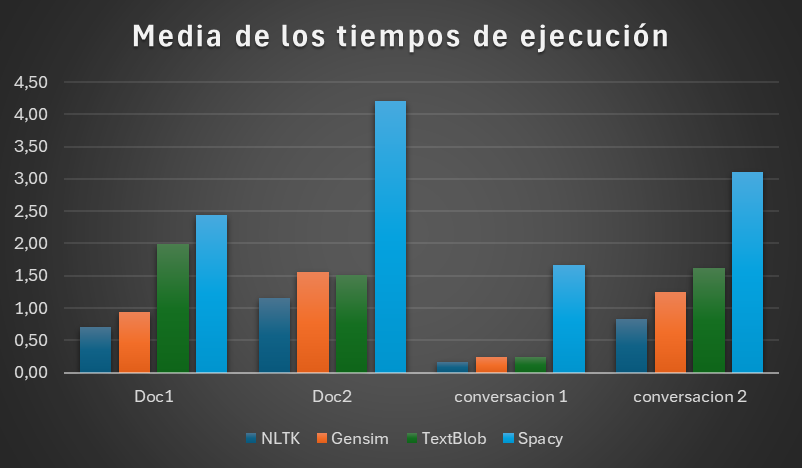
\includegraphics[scale=0.25]{imagenes/grafico_tiempos_procesado}
        \caption{Tiempos de procesamiento por fragmento}
        \label{fig:grafico_tiempos_procesado}
    \end{figure}


    \section{Análisis de resultados}\label{sec:analisis-de-resultados}
    En esta sección se analizarán los resultados obtenidos en la normalización de los textos de prueba.
    Como hay mucha información, los datos relativos a cada librería se han puesto como archivos adjuntos.
    En el \autoref{app:a} se pueden ver los textos de prueba y en el \autoref{sec:salidanormalizacion} se pueden ver los resultados de la normalización.

    \subsection{Bag of Words}\label{subsec:bow}
    En general, los resultados obtenidos para el \textit{Bag of Words} han sido bastante buenos.
    Los resultados antes y después se pueden resumir en:
    \itemize{
        \item Se ha reducido la dimensionalidad (número de palabras) del texto.
        \item Se han eliminado (en la mayoría de los casos) caracteres no deseados como puntuación y números.
        \item Se han lematizado y stemmerizado las palabras, reduciendo la dimensionalidad.
        \item Se ha corregido la ortografía, evitando falsas diferencias.
    }

    \subsection{Análisis de sentimientos}\label{subsec:sentimientos}
    En general, los resultados obtenidos para el análisis de sentimientos han sido buenos.
    Cuando se ha aplicado el análisis de sentimientos a los textos normalizados, se ha obtenido una mejoría sustancial en la precisión de los resultados.

    El caso en el que más se ha notado la diferencia ha sido en el de NLTK \autoref{fig:nltk-sentimientos}.
    En este, se ha pasado de un patrón más negativo y con valores extremos a un patrón más equilibrado y realista.
    Además, este se ajusta más a la realidad del texto.

    En general, se puede afirmar que la normalización de los textos ha mejorado la precisión de los análisis de sentimientos.


    \subsection{Name Entity Recognition y POS}\label{subsec:ner-pos}
    Para esta sección hay que especificar que:
    \itemize
    {
    \item Spacy ha usado a NLTK para POS y NER.
    \item TextBlob no tiene soporte para NER.
    \item Gensim no tiene soporte para NER ni POS.
    }

    Una vez dicho esto, se puede afirmar que los resultados obtenidos para POS y NER
    han sido buenos en el caso previo a la normalización.
    Se puede observar que tras normalizar, los resultados empeoran.
    Esto se debe a que la normalización ha eliminado palabras clave y ha cambiado la estructura de las frases.
    La pérdida de información ha hecho que los resultados sean menos precisos.



    \begin{figure}
        \vspace{1.5pt}
        \centering
        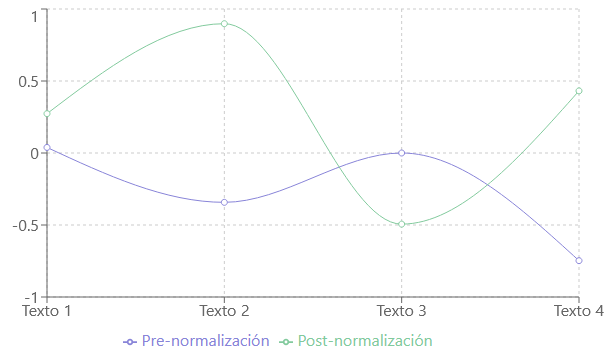
\includegraphics[scale=0.25]{imagenes/nltk-sentimientos}
        \caption{Sentimientos detectados por spacy antes y después de normalizar}
        \label{fig:nltk-sentimientos}
    \end{figure}





%        \label{fig:menorOigual}
%    \end{figure}


%    \clearpage
%    \begin{figure}
%        \centering
%        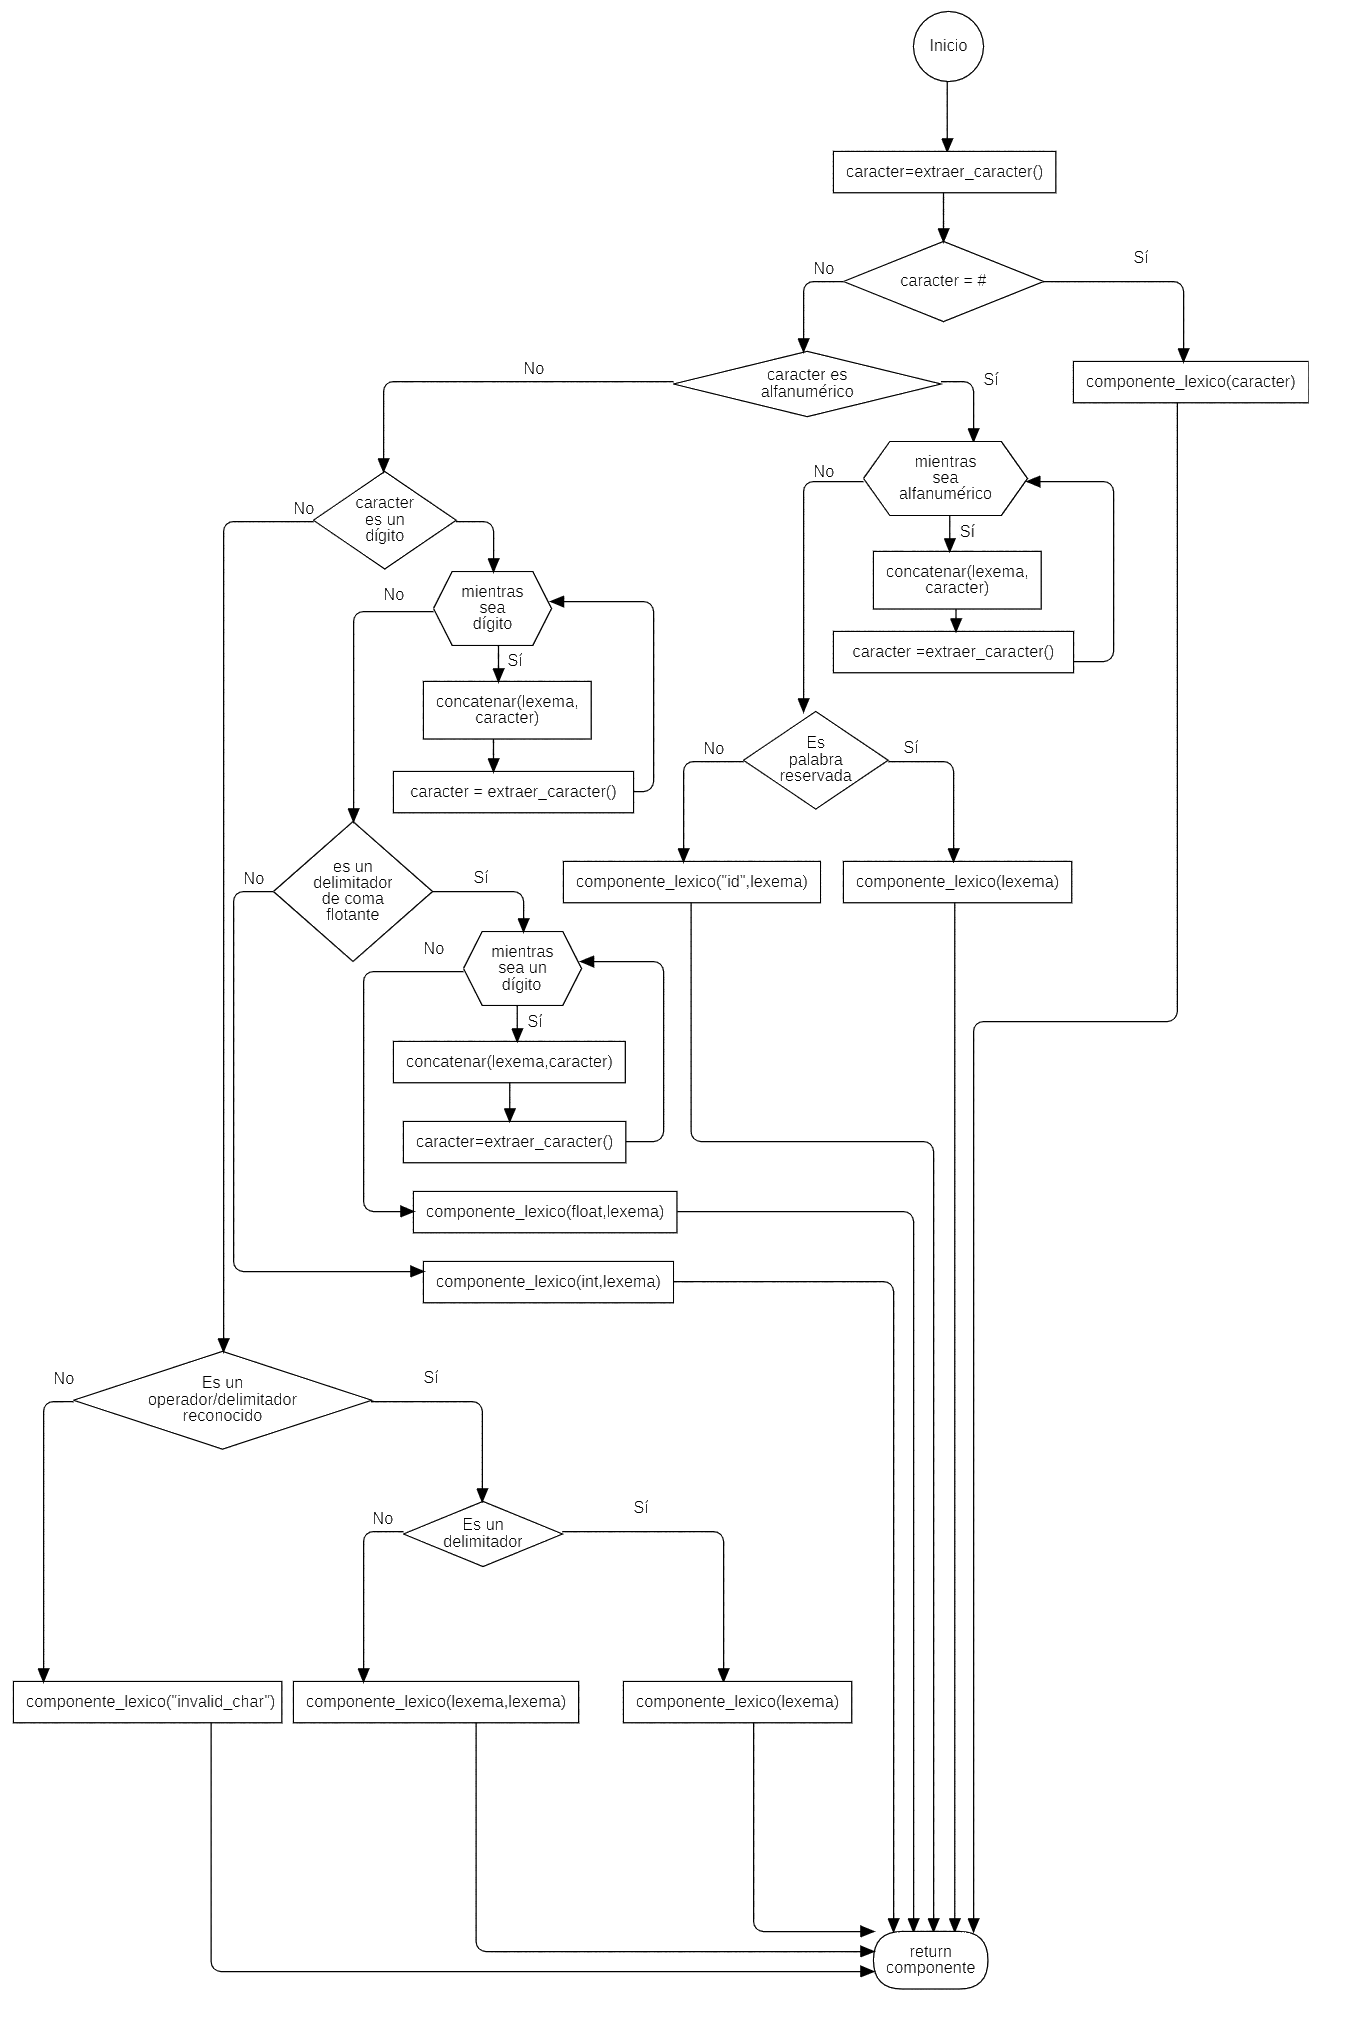
\includegraphics[width=1.00\linewidth]{diagramaFlujoDecisionCaracteresFinal}
%        \caption{Diagrama de flujo para la creación de un token}
%        \label{fig:diag 1}
%    \end{figure}


    \section{Conclusiones y algunas reflexiones}\label{sec:conclusiones-y-algunas-reflexiones}

    En general, podemos afirmar que el procesamiento de texto es una tarea que aunque añade
    tiempo al procesamiento, mejora la calidad de los resultados en la mayoría de los casos.

    Recapitulando al informe previo~\autocite{marcelo.informe1}, podemos extraer algunas reflexiones:
    En una primera instancia, puede parecer lo mismo el procesado de texto por un compilador que por una librería de procesamiento de texto,
    per esto rápidamente se desvanece.
    Esto se debe a varios factores:
    \begin{itemize}
    {
        \item El compilador es generalmente determinista, es decir, sigue unas «reglas»(producciones) fijas y predefinidas,
        mientras que los modelos de procesamiento de texto son estadísticos y usan patrones y probabilidades.
        \item Los compiladores se centran en aspectos formales y comprueban la corrección de un texto, mientras que los modelos de lenguaje natural se centran en el significado y contexto.
        Esto permite que puedan detectar errores y hacer sugerencias.
        \item Un modelo de lenguaje NO puede asegurar la compilabilidad de un texto, ya que no tiene en cuenta aspectos formales y puede «alucinar» debido a su naturaleza estadística.
        \item Un compilador solo compila, mientras que un modelo de lenguaje puede hacer muchas cosas, desde análisis de sentimientos hasta traducción.
    }
\end{itemize}
    Se puede extraer que su diferencia fundamental radica en la naturaleza de sus respuestas.
    Un compilador busca dar «feedback» sobre la corrección de un código,
    mientras que un modelo de lenguaje puede ofrecer sugerencias sobre mejoras, explicar el contexto, o incluso detectar zonas subóptimas de ese mismo código.
    Esto tiene implicaciones en la forma de trabajar con ellos,
    permitiendo que se complementen y se usen en conjunto para obtener mejores resultados.



    En el caso específico de los modelos NLP entrenados específicamente para un código, pueden salir ciertas implicaciones.

    A nivel ético,
    primeramente, el hecho de que hayan sido entrenados con un código específico puede llevar a que tengan sesgos, ya que el código puede tenerlos.
    Estos podría a contribuir a malas prácticas, tanto a nivel de optimización como a nivel social,
    llegando a crear algoritmos que tengan sesgos raciales, machistas o aporofóbicos.

    El entrenamiento de estos modelos  también es motivo de preocupación, ya que muchas veces no se respeta la privacidad de los datos.
    Esto lleva a que se puedan obtener datos sensibles de los usuarios y se puedan usar de forma maliciosa o utilizar fragmentos de código con copyright.

    A nivel práctico,
    El código generado por estos modelos también puede ser motivo de preocupación.
    No se asegura que esté al último standard, que sea seguro o que sea eficiente.
    Además, no se puede pedir responsabilidades a un modelo de lenguaje, ya que no tiene capacidad de decisión.
    Por lo que la responsabilidad recae en el usuario que lo use.

    El uso sistematizado necesita de una supervisión humana para asegurar que los resultados son los esperados y que no se están cometiendo errores.
    Además, los modelos de lenguaje no suelen usar las opciones más eficientes, por lo que se puede perder rendimiento en el código generado.

    Hay que tener en cuenta, que el entrenamiento se basa en el código publicado en repositorios públicos.
    Esto puede y es positivo, pero también puede ser negativo, ya que por la naturaleza de internet, habrá mucho más código subóptimo que código óptimo.

    En resumen, los modelos de lenguaje son una herramienta muy potente, pero que necesita de una supervisión humana para asegurar que los resultados son los esperados y que no se están cometiendo errores.
    Además, no se puede pedir responsabilidades a un modelo de lenguaje, ya que no tiene capacidad de decisión.
    Esta recae en el usuario que lo use.

    \newpage

%------------------------------------------------


%------------------------------------------------


%----------------------------------------------------------------------------------------
%	Referencias
%----------------------------------------------------------------------------------------

%    \bibliographystyle{IEEEtran}
    \printbibliography

    \clearpage


    \makeatletter
    \newcommand\appendix@section[1]{%
        \refstepcounter{section}%
        \orig@section*{Apéndice \@Alph\c@section: #1}%
        \addcontentsline{toc}{section}{Apéndice \@Alph\c@section: #1}%
    }
    \let\orig@section\section
    \g@addto@macro\appendix{\let\section\appendix@section}
    \makeatother


    \appendix


    \section{Textos de prueba para normalizar}\label{sec:textosAnormalizar} \label{app:a}

    \subsection{Texto 1 de prueba}\label{subsec:texto1}
    Colia tookw the prince to a public-house in the Litaynaya, not far off.
    In one of the side rooms there sat at a table—looking like one of the
    regular guests of the establishment Ardalion Alexandrovitch, with a
    bottle before him, and a newspaper on his knee.
    He was waiting for the
    prince, and no sooner did the latter appear than he began a long
    harangue about something or other; but so far gone was he that the
    prince could hardly understand a word.

    \subsection{Texto 2 de prueba}\label{subsec:texto2}
    But why recall all this?
    There was insanity on both sides.
    For him, the
    prince, to love this woman with passion, was unthinkable.
    It would be
    cruel and inhuman.
    Yes.
    Rogojin is not fair to himself; he has a large
    heart; he has aptitude for sympathy.
    When he learns the truth, and
    finds what a pitiable being is this injured, broken, half-insane
    creature, he will forgive her all the torment she has caused him.
    He
    will become her slave, her brother, her friend.
    Compassion will teach
    even Rogojin, it will show him how to reason.
    Compassion is the chief
    law of human existence.
    Oh, how guilty he felt towards Rogojin!
    And,
    for a few warm, hasty words spoken in Moscow, Parfen had called him
    ``brother'', while he—but no, this was delirium!
    It would all come right!
    That gloomy Parfen had implied that his faith was waning; he must
    suffer dreadfully.
    He said he liked to look at that picture; it was not
    that he liked it, but he felt the need of looking at it.
    Rogojin was
    not merely a passionate soul; he was a fighter.
    He was fighting for the
    restoration of his dying faith.
    He must have something to hold on to
    and believe, and someone to believe in.
    What a strange picture that of
    Holbein’s is!
    Why, this is the street, and here’s the house, No. 16.

    \subsection{Texto 3 de Prueba}\label{subsec:texto3}

    The prince pulled a letter out of his pocket.

    ``Is he raving?'' said the general.
    ``Are we really in a mad-house?''

    There was silence for a moment.
    Then Ptitsin spoke.

    \subsection{Texto 4 de prueba}\label{subsec:texto4}

    ``Bravo!'' said Ferdishenko.
    Ptitsin laughed too, though he had been very
    sorry to see the general appear.
    Even Colia laughed and said, ``Bravo!''

    ``And I was right, truly right,'' cried the general, with warmth and
    solemnity, `` if cigars are forbidden in railway carriages, poodles
    are much more so.''

    ``Well, and what did the lady do?'' asked Nastasia, impatiently.

    ``She—ah, that’s where all the mischief of it lies!'' replied Ivolgin, frowning.
    ``Without a word, as it were, of warning, she slapped me on the cheek!
    An extraordinary woman!''

    \newpage

    \section {Salida de normalización}\label{sec:salidanormalizacion}
    Aquí se muestra la salida de la normalización de los textos de prueba.
    Las cadenas mostradas son la unión de los tokens normalizados.

    \subsection{NLTK}\label{subsec:nltk_out}
    \begin{itemize}
        \item Texto 1: colin took princ public hous litaynaya far in one side room sat tabl look like one regular guest establish ardalion alexandrovich bottl newspap knee he wait princ sooner latter appear began long harangu someth far gone princ could hard understand word
        \item Texto 2: but recal there insan side for princ love woman passion unthink it would cruel inhuman yes rogojin fair larg heart aptitud sympathi when learn truth find potabl injur broken half insan creatur forgiv torment caus he becom slave brother friend compass teach even rogojin show reason compass chief law human exist oh guilti felt toward rogojin and warm hasti word spoken moscow parent call brother delirium it would come right that gloomi parent impli faith wane must suffer dread he said like look pictur like felt need look rogojin mere passion soul fighter he fight restor die faith he must someth hold believ someon believ what strang pictur holbein whi street hous no
        \item Texto 3: the princ pull letter pocket is said general are realli mad hous there silenc moment then pitkin spoke
        \item Texto 4: bravo said ferdishenko pitkin laugh though sorri see general appear even colin laugh said bravo and i right truli right cri general warmth solemn cigar forbidden railway carriag noodl much well ladi ask natasha impati she ah mischief lie repli violin drown without word warn slap cheek an extraordinari woman
    \end{itemize}

    \subsection{spaCy}\label{subsec:spaCy_out}
    \begin{itemize}
        \item Texto 1: colia tookw prince public house city far room sit table look like regular guest establishment alexandrovitch bottle newspaper knee wait prince soon appear begin long argument far go prince hardly understand word
        \item Texto 2: recall insanity side prince love woman passion insane cruel brutal yes fair large heart ask sympathy learn truth find terrible injure broken half insane creature forgive torment cause slave brother friend compassion teach reason compassion chief law human existence oh guilty feel warm happy word speak moscow call brother come right man imply faith fail suffer terribly say like look picture like feel need look Julian merely passionate soul fighter fight restoration die faith hold believe believe strange picture John street house
        \item Texto 3: prince pull letter pocket say say general mad house silence moment speak
        \item Texto 4: no say ferdishenko ptitsin laugh sorry general appear laugh say no right truly right cry general warmth sincerity cat forbid railway carriage lady ask nastasia impatiently ah mystery lie reply Polly frown word warning slap cheek extraordinary woman
    \end{itemize}

    \subsection{GenSim}\label{subsec:gensim_out}
    \begin{itemize}
        \item Texto 1: colin princ public hous litaynaya far room sit table—look like regular guest establish ardalion alexandrovich bottl newspap knee wait princ sooner appear begin long harangu far princ hardli understand word
        \item Texto 2: recal insan side princ love woman passion unthink cruel inhuman ye rogojin fair larg heart aptitud sympathi learn truth potabl injur broken half insan creatur forgiv torment caus slave brother friend compass teach rogojin reason compass chief law human exist guilti feel rogojin warm hasti word speak moscow parent “brother he—but delirium come right gloomi parent impli faith wane suffer dread like look pictur like feel need look rogojin mere passion soul fighter fight restor die faith hold believ believ strang pictur holbein’ street here’ hous
        \item Texto 3: princ pull letter pocket “i have gener “are mad hous silenc moment pitkin spoke
        \item Texto 4: “bravo ferdishenko pitkin laugh sorri gener appear colin laugh said “bravo “and right truli right gener warmth solemnli “for cigar forbid railwai carriag noodl “well ladi ask natasha impati “she—ah that’ mischief li repli violin drown “without word warn slap cheek extraordinari woman
    \end{itemize}

    \subsection{TextBlob}\label{subsec:textblob_out}
    \begin{itemize}
        \item Texto 1: solid took princ public-hous litaynaya far one side room sat table—look like one regular guest establish ardalion alexandrovitch bottl befor newspap hi knee wa wait princ sooner latter appear began long harangu someth far gone wa princ could hardli understand word
        \item Texto 2: whi recal thi wa insan side princ love thi woman passion wa unthink would cruel inhuman ye rogojin fair ha larg heart ha aptitud sympathi learn truth find pitiabl thi injur broken half-insan creatur forgiv torment ha caus becom slave brother friend compass teach even rogojin show reason compass chief law human exist oh guilti felt toward rogojin warm hasti word spoken moscow garden call “ brother ” he—but thi wa delirium would come right gloomi garden impli hi faith wa wane must suffer dread said like look pictur wa like felt need look rogojin wa mere passion soul wa fighter wa fight restor hi die faith must someth hold believ someon believ strang pictur holbein ’ whi thi street ’ hous
        \item Texto 3: princ pull letter hi pocket “ rave ” said gener “ realli mad-hous ” wa silenc moment ptitsin spoke
        \item Texto 4: “ bravo ” said ferdishenko ptitsin laugh though veri sorri see gener appear even solid laugh said “ bravo ” “ wa right truli right ” cri gener warmth solemn “ cigar forbidden railway carriag peopl much ” “ well ladi ” ask nastasya impati “ the—ah ’ mischief lie ” repli ivolgin frown “ without word warn slap cheek extraordinari woman ”

    \end{itemize}

\end{document}